\section{DCD}
A data context diagram is used in order to figure out more of the requirements asked by the client. The data context diagram is made with the rules of Yourdon. The DCD is included in \autoref{fig:DCD}.

\begin{figure}[H]
    \hspace{-2.5cm}
    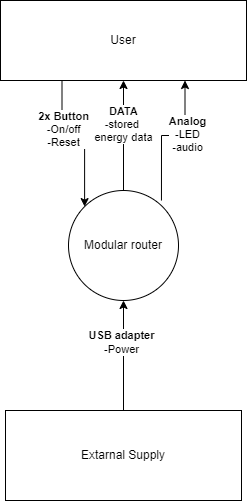
\includegraphics[width=20cm]{Images/Definition phase/DCD.drawio.png}
    \caption{DCD}
    \label{fig:DCD}
\end{figure}

\newpage
\section{Requirements}
In this chapter the Requirements will be listed. For the requirements the MoSCoW method is used. The MoSCoW method makes use of priority. In \autoref{tab:moscow_abbreviations} the abbreviations are listed.

\begin{table}[H]
\centering
    \begin{tabular}{l p{8cm}}
        \textbf{Abbreviation} & \textbf{Meaning} \\
        MH & Must Have | This requirement must be developed and has to work in the end product\\
        & \\
        SH & Should Have | It isn't mandatory to make, but it would be preferred if it is developed\\
        & \\
        CH & Could Have | It isn't mandatory, but if there is time, it will be developed\\
        & \\
        WH & Won't Have |isn't necessary\\
    \end{tabular}
    \caption{MoSCoW abbreviations}
    \label{tab:moscow_abbreviations}
\end{table}

The requirements will be listed in the format listed below.\\

\newRequirement{Number}{MoSCoW priority}{\emph{explanation}}


\subsection{Wireless/modular}
%opties hiervoor
The router will be modular by using wireless communication as to create a mesh network. In this chapter the requirements for the wireless and modular will be given.



\subsection{Connections}
This chapter will give the requirements for the connections that are necessary. 

\newRequirement{2.1}{MH}{
    The router needs a working connection for Ethernet.
}

\newRequirement{2.2}{MH}{
    The Router needs a working connection that can connect with a smart meter
}

\newRequirement{2.3}{MH}{
    The Router needs a working connection for the rs485 protocol
}

\newRequirement{2.4}{MH}{
    The microcontroller needs to be able to be flashed
}

\newRequirement{2.5}{CH}{
    The router can have a working USB connection.
}

\subsection{User interface}
This chapter is created for the user interface so the router can be easily applied.
\newRequirement{3.1}{SH}{
    The Router can have a reset button.
}
\newRequirement{3.2}{CH}{
    The Router can have LED's which show the status of the Router.
    }
\newRequirement{3.3}{CH}{
    The Router can have a display that shows the used power.
}
\newRequirement{3.4}{MH}{
    The Router must have an on and off option.
}
\newRequirement{3.5}{CH}{
    The Router can have a small speaker that warns the user if something went wrong.
}

\subsection{Supply/transformer}
This will give the requirements for the transformer so the router can be plugged in and have the right amount of voltage and current for the controller.

\newRequirement{4.1}{MH}{
    The Router will need short circuit protection if it overloads or if someone connects the wrong input.
}

\newRequirement{4.2}{MH}{The input of the system will be 5 V}

\newRequirement{4.3}{MH}{Transform the input voltage to the correct voltage so the microcontroller can use it.}

\subsection{Data}
The Router will also need a storage unit that can store the energy information.

\newRequirement{5.1}{SH}{
    The Router should have a A compute module in order to store more energy data. 
}

\newRequirement{5.2}{WH}{
    The code wont be written in order to store the data.
}
%wat zijn mogelijkheden voor hardware ivm de modular dinggetje.


\subsection{Non functional requirements}
Next to the normal requirements there are also non functional requirements. This entails that these requirements wont have any functionality.

\newNFRequirement{1.1}{MH}{
    Bill of material for the end product PCB.
}

\newNFRequirement{1.2}{SH}{
    The Router needs an outside case in which the PCB fits.
}


\section{Acceptance test}
\subsection{Test setup}
\label{sec:Test_setup}
In order to test a requirement there needs to be a test setup that can test the finished project properly. The test setup includes the room in which the requirements are tested and the equipment that is necessary.

\subsubsection{Test room}
The test room will be the room at Crownstone. In which the the necessary equipment is located.

\subsubsection{Equipment}

To test the completed product the necessary equipment is listed below

\begin{itemize}
    \item An adapter
    \item A laptop to read out the results
    \item A multi meter to test different voltages
\end{itemize}

\newAcceptanceTest{\reqRef{REQ1.1},\reqRef{REQ1.2} and \reqRef{REQ1.3}}
{See \nameref{sec:Test_setup}}
{A package of data}
{The same package of data on another device}
{\begin{itemize}
    \item The package can be received with a range of 20 meters.
    \item The data package needs to be the same
    \item Bluetooth and WiFi needs to be used in order to send the package
\end{itemize}}
{\begin{enumerate}
    \item Get a device(s) that can be connected to with WiFi and/or Bluetooth
    \item Put the router on.
    \item Make sure the WiFi device is connected to the same WiFi  network
    \item Make sure the Bluetooth device is connected to the router
    \item Send a package through the device with WiFi
    \item Check if the package arrived correctly
    \item Now do the same with Bluetooth
    \item Check the maximum range of the Bluetooth and WiFi and fill it in below.
\end{enumerate}

\begin{tabular}{c|c}
    Communication type & Range \\\hline
    \multirow{2}{3em}{WiFi} & \\& \underline{\hspace{3cm}}\\
    \multirow{2}{4em}{Bluetooth} &\\& \underline{\hspace{3cm}}\\
\end{tabular}}

\newAcceptanceTest{\reqRef{REQ2.1}, \reqRef{REQ1.5}, \reqRef{REQ1.8}, \reqRef{REQ1.4}}
{See \nameref{sec:Test_setup}}
{A package send from a laptop with an Ethernet cable}
{The same package at the router}
{\begin{itemize}
    \item The package needs to be delivered through Ethernet
    \item The package needs to be the same
\end{itemize}}
{\begin{enumerate}
    \item Start up the laptop and the router
    \item Connect an Ethernet cable to the router
    \item Ready the package
    \item send the package
    \item Check if the package is the correct
    \item Do the same for the modular connection
    \item Connect a wrong rs485 connection to the Ethernet modular connection
    \item Check if the system rejects the rs485
\end{enumerate}}

\newAcceptanceTest{\reqRef{REQ2.2}, \reqRef{REQ1.7}}
{See \nameref{sec:Test_setup}}
{A smart meter measurement}
{Smart meter data}
{\begin{itemize}
    \item Correct measurement
    \item Use different smart meters
\end{itemize}}
{\begin{enumerate}
    \item Connect the smart meter to the router
    \item Make sure the smart meter is on
    \item Activate the router
    \item Read out the data that was sent from the smart meter to the router.
    \item Check with another device if the data is read correct
    \item Do the same for the modular connection
\end{enumerate}}

\newAcceptanceTest{\reqRef{REQ2.3}, \reqRef{REQ1.6}}
{See \nameref{sec:Test_setup}}
{Data from the router}
{The received data at a laptop}
{\begin{itemize}
    \item The data has been sent correctly
    \item The data is correct
\end{itemize}}
{\begin{enumerate}
    \item Connect the router to the laptop via the rs485 protocol.
    \item Send the data
    \item Check if the data has been successfully transferred
    \item Do the same for the modular connection
\end{enumerate}}

\newAcceptanceTest{\reqRef{REQ2.4}, \reqRef{REQ2.5}}
{See \nameref{sec:Test_setup}}
{Micro-USB connected to a laptop flashing code}
{Working microcontroller}
{\begin{itemize}
    \item The microcontroller needs to be flashed
    \item The USB connection works
\end{itemize}}
{\begin{enumerate}
    \item Activate the router
    \item Ready the laptop
    \item Flash code with a command to the microcontroller
    \item Check if the USB port works
\end{enumerate}}

\newAcceptanceTest{\reqRef{REQ3.1}, \reqRef{REQ3.2}, \reqRef{REQ3.3}, \reqRef{REQ3.4}, \reqRef{REQ3.5}}
{See \nameref{sec:Test_setup}}
{\begin{itemize}
    \item User input
\end{itemize}}
{\begin{itemize}
    \item A sound
    \item Visual status router
    \item System reset
    \item System turns on/off
\end{itemize}}
{\begin{itemize}
    \item The system has to reset
    \item The LED's need to turn on for the correct statusses.
\end{itemize}}
{\begin{enumerate}
    \item Turn the router on by pushing the button.
    \item See if the light turns on to display the on status.
    \item Press the reset button
    \item See if the router resets.
    \item Attach a module wrongly
    \item See if the Speaker gives of a sound
\end{enumerate}}

\newAcceptanceTest{\reqRef{REQ4.1} and \reqRef{REQ4.2} and \reqRef{REQ4.3}}
{See \nameref{sec:Test_setup}}
{\begin{itemize}
    \item 5V
    \item More than 5V
\end{itemize}}
{\begin{itemize}
    \item The microcontroller works
    \item The Router will shut down
\end{itemize}}
{\begin{itemize}
    \item When a too high current is put in the system needs to shut down.
    \item The 5V needs to transform into 3.3V
\end{itemize}}
{\begin{enumerate}
    \item Put the 5V into the router
    \item Check if 5V is measured with a multimeter
    \item Check if the 5V is transformed into 3.3V to power the microcontroller
    \item Before putting in more make sure you can pull out the supply if it doesn't work.
    \item Put in more than 5V
    \item Check if the system shut down
\end{enumerate}}
 
\newAcceptanceTest{\reqRef{REQ5.1}, \reqRef{REQ5.2}}
{See \nameref{sec:Test_setup}}
{Storage data}
{Storage data}
{\begin{itemize}
    \item The data needs to be stored in an outside source
\end{itemize}}
{\begin{enumerate}
    \item Startup the router
    \item Send a packet to router
    \item Make sure the packet is stored in the external storage
    \item Check if the packet is stored correctly
\end{enumerate}}

\section{Traceability requirements}
\begin{table}[H]
    \centering
    \begin{tabular}{|l|p{1.2cm}|p{1.2cm}|p{1.2cm}|p{1.2cm}|p{1.2cm}|p{1.2cm}|p{1.2cm}|p{1.2cm}|}\hline
        \textbf{Requirements}&\textbf{Test case 1}&\textbf{Test case 2}&\textbf{Test case 3}&\textbf{Test case 4}&\textbf{Test case 5}&\textbf{Test case 6}&\textbf{Test case 7}&\textbf{Test case 8}\\\hline
        \reqRef{REQ1.1}&\vink& & & & & & &\\\hline
        \reqRef{REQ1.2}&\vink& & & & & & &\\\hline
        \reqRef{REQ1.3}&\vink& & & & & & &\\\hline
        \reqRef{REQ1.4}& &\vink& & & & & &\\\hline
        \reqRef{REQ1.5}& &\vink& & & & & &\\\hline
        \reqRef{REQ1.6}& & & &\vink& & & &\\\hline
        \reqRef{REQ1.7}& & &\vink& & & & &\\\hline
        \reqRef{REQ1.8}& &\vink& & & & & &\\\hline
        \reqRef{REQ2.1}& &\vink& & & & & &\\\hline
        \reqRef{REQ2.2}& & &\vink& & & & &\\\hline
        \reqRef{REQ2.3}& & & &\vink& & & &\\\hline
        \reqRef{REQ2.4}& & & & &\vink& & &\\\hline
        \reqRef{REQ2.5}& & & & &\vink& & &\\\hline
        \reqRef{REQ3.1}& & & & & &\vink& &\\\hline
        \reqRef{REQ3.2}& & & & & &\vink& &\\\hline
        \reqRef{REQ3.3}& & & & & &\vink& &\\\hline
        \reqRef{REQ3.4}& & & & & &\vink& &\\\hline
        \reqRef{REQ3.5}& & & & & &\vink& &\\\hline
        \reqRef{REQ4.1}& & & & & & &\vink&\\\hline
        \reqRef{REQ4.2}& & & & & & &\vink&\\\hline
        \reqRef{REQ4.3}& & & & & & &\vink&\\\hline
        \reqRef{REQ5.1}& & & & & & & &\vink\\\hline
        \reqRef{REQ5.2}& & & & & & & &\vink\\\hline
    \end{tabular}
    \caption{Traceability requirements}
    \label{tab:Traceability_requirements}
\end{table}
